\documentclass{beamer}

\usepackage[utf8]{inputenc}
\usepackage[russian]{babel}
\usepackage{hyperref}
\usepackage{graphicx}
\usepackage{listings}

\usetheme{Warsaw}
\usecolortheme{lily}
\useoutertheme[subsection=false]{smoothbars}
\useinnertheme{circles}
\setbeamertemplate{footline}[page number]{}
\setbeamertemplate{navigation symbols}{}

\renewcommand{\figurename}{} 

\title{Архитектура ЭВМ}
\subtitle{Лекция 3. Что такое x86?}
\author{к.ф.-м.н. Филонов Павел Владимирович \\ filonovpv@gmail.com}
\date{15 сентября 2013 г.}


\institute[МГТУ ГА] 
{
    Московский Государственный Технический Университет \\
    Гражданской Авиации
}
\begin{document}
    \frame{\titlepage}
    \section{Intel}
    \subsection{}
    \begin{frame}{Повестка дня}
    	\begin{enumerate}
    	\pause
    	\item Краткая история процессоров Intel
    	\pause
    	\item Архитектура x86
    	\pause
    	\item Что означают следующие надписи: x86-64, i386, IA-32, IA-64?
    	\pause
    	\item Кто пишет понятней: AT\&T или Intel?
    	\pause
    	\item NASM --- наше всё!
    	\pause
    	\item Макросы нам помогут!
    	\end{enumerate}
    \end{frame}
    \begin{frame}{Intel 4004 --- 1971 год}
    \begin{columns}
    	\column{0.4\linewidth}
    	\includegraphics[width=0.7\linewidth]{fig/Intel_4004.jpg}
    	\footnotesize

    	Основные характеристики:
    	\begin{itemize}
    		\item Тактовая частота 92,6 кГц
    		\item Гарвардская архитектура
    		\item Объём адресуемой памяти: 640 байт
    		\item 16 4-х битных регистров
    		\item Число инструкций --- 46
    		\item Число транзисторов --- 2250 
    	\end{itemize}
    	\column{0.6\linewidth}
    	\begin{figure}
    		\includegraphics[width=\linewidth]{fig/4004_arch.png} \\
    		Блок-схема
    	\end{figure}
    \end{columns}
    \end{frame}
    \begin{frame}{Intel 8080 --- 1974 год}
    \begin{columns}
    	\column{0.4\linewidth}
    	\includegraphics[width=0.8\linewidth]{fig/Intel_8080.jpg}
    	\footnotesize

    	Основные характеристики:
    	\begin{itemize}
    		\item Тактовая частота: 2 мГц
    		\item Прингстонская архитектура
    		\item Объём адресуемой памяти: 64 Кбайт
    		\item 7 8-ми битных регистров
    		\item Число инструкций --- 80
       		\item Число транзисторов --- 6000  
    	\end{itemize}
    	\column{0.6\linewidth}
    	\begin{figure}
    		\includegraphics[width=\linewidth]{fig/Altair_8800.jpg}

    		Altair 8800
    	\end{figure}
    \end{columns}
    \end{frame}
    \begin{frame}{Intel 8088 --- 1979 год}
    \begin{columns}
    	\column{0.4\linewidth}
    	\includegraphics[width=0.8\linewidth]{fig/Intel_8088.jpg}
    	\footnotesize

    	Основные характеристики:
    	\begin{itemize}
    		\item Тактовая частота: 5 мГц
    		\item Объём адресуемой памяти: 1 Мбайт
    		\item 8 16-ти битных регистров
    		\item Число инструкций --- 98
    		\item Число транзисторов --- 29000  
    	\end{itemize}
    	\column{0.6\linewidth}
    	\begin{figure}
    		\includegraphics[width=\linewidth]{fig/IBM_PC.jpg}

    		IBM PC
    	\end{figure}
    \end{columns}
    \end{frame}
    \begin{frame}{Intel 80386 (i386) --- 1985 год}
    \begin{columns}
    	\column{0.4\linewidth}
    	\includegraphics[width=0.7\linewidth]{fig/i386.png}
    	\footnotesize

    	Основные характеристики:
    	\begin{itemize}
    		\item Тактовая частота: 16, 20,25,33,40 мГц
    		\item Объём адресуемой памяти: 4 Гбайт
    		\item 8 32-х битных регистров
    		\item Число инструкций --- 150 (x86 или IA-32)
    		\item Число транзисторов --- 275000
    	\end{itemize}
    	\column{0.6\linewidth}
    		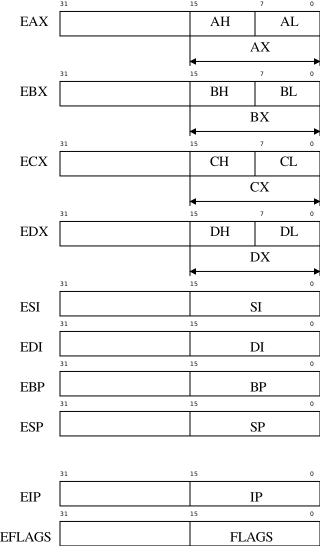
\includegraphics[width=0.7\linewidth]{fig/x86_regs.pdf}

    \end{columns}
    \end{frame}
    \begin{frame}{И остальные модели}
    	\begin{itemize}
    		\item {\bf i486} --- математический сопроцессор (FPU), кеш L1, L2
    		\item {\bf Pentium} --- суперскалярная архитектура, предсказание ветвлений, раздельное кеширование кода и данных
    		\item {\bf Pentium II} --- SIMD MMX инструкции
    		\item {\bf Pentium III} --- RISC-ядро, SSE (Streaming SIMD Extensions)
    		\item {\bf Pentium 4} --- Hyper-threading, SSE2, SSE3, EMT64T(x86-64 или IA-64)
    		\item {\bf Pentium D} --- 2 ядра
    		\item {\bf Core 2} --- 1,2,4 ядра, VT-x, SSSE3
    		\item {\bf Core i3,i5,i7} --- Hyper-threading, встроенный графический процессор, SSE4

    	\end{itemize}
    \end{frame}
\end{document}